\newpage
\section{Test 7}
\label{Sec:test_7}

In the seveth test setting rover is dropped onto a horizontal plane.
An obstacle in the form of a horizontal step of height $0.1m$ has been set in front of the rover.
At certain point of time ($t = 10s$) rover starts moving towards the step and crosses it mounting on the higher plane.
Friction coefficient has been set to 0.6. Restitution coefficient (normal) has been set to 0.1. 

\begin{figure}[H]
  \centering
    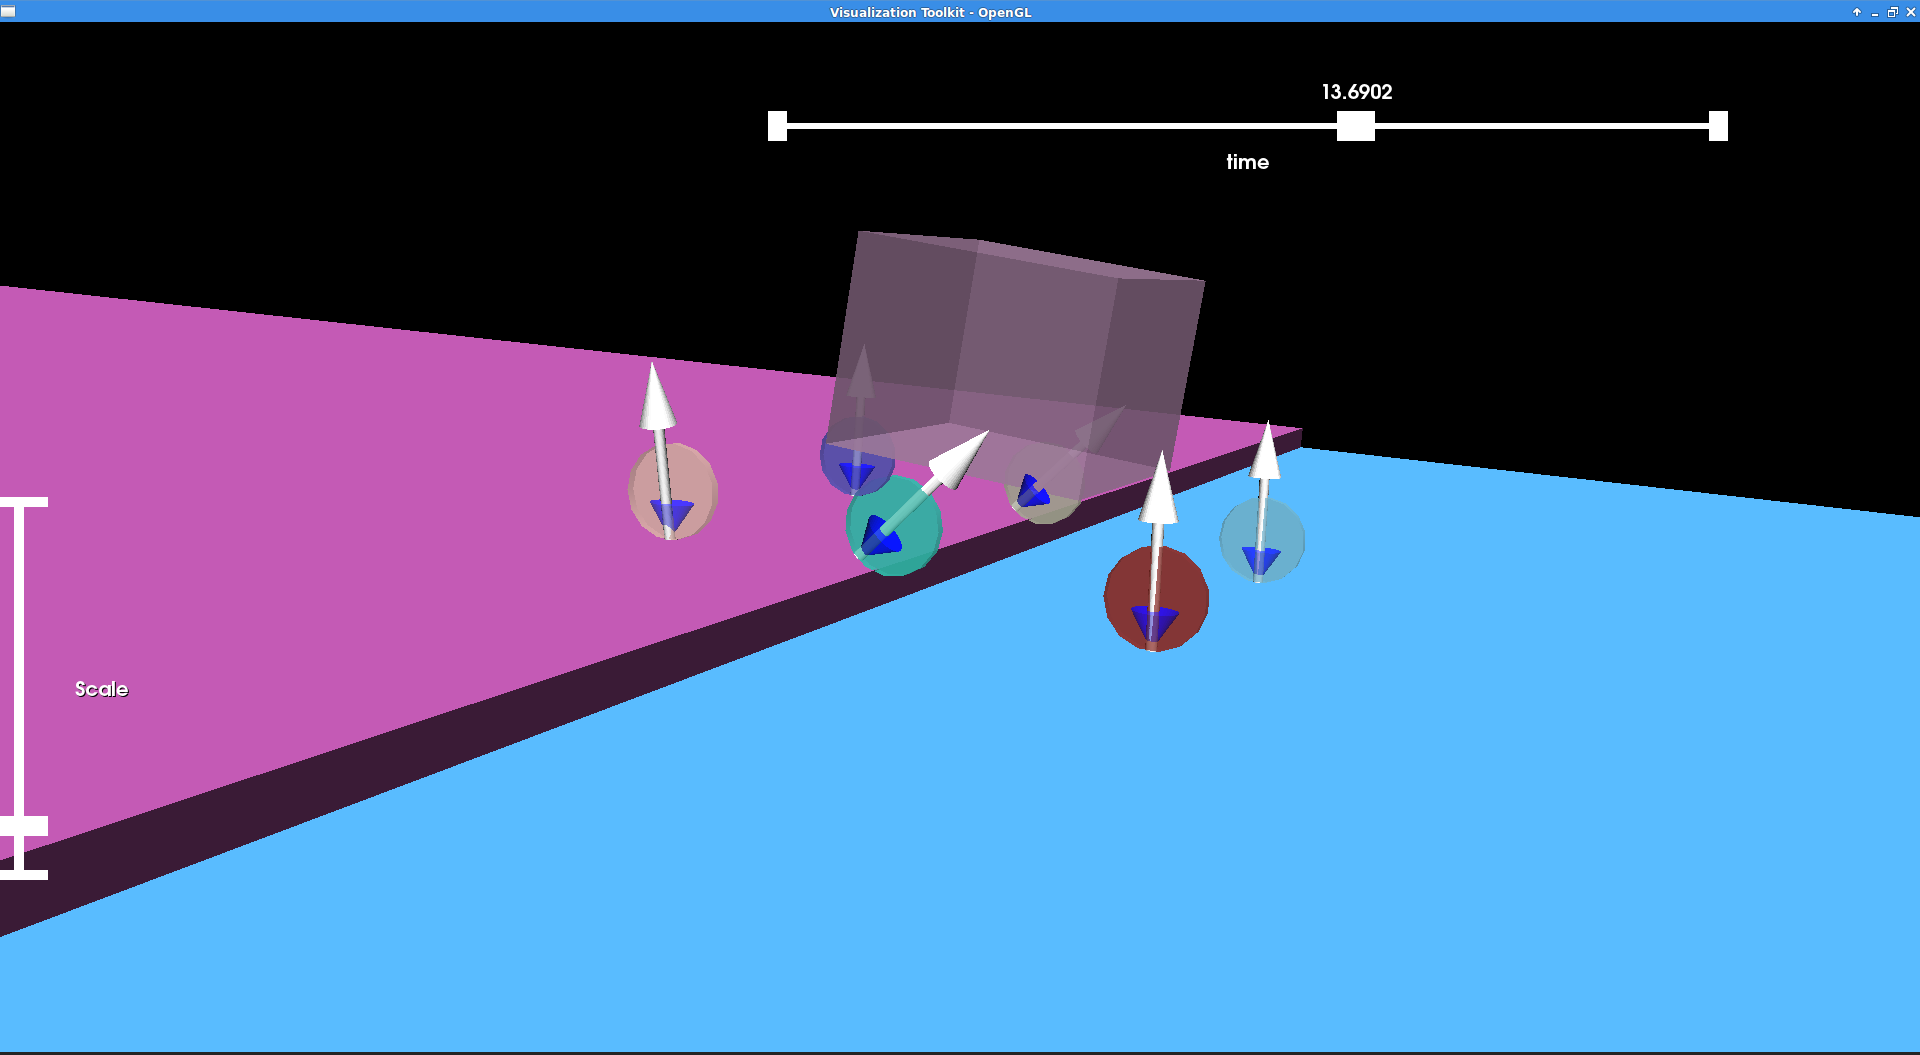
\includegraphics[width=0.8\textwidth]{run_7}
  \caption{Seventh test scenario}
\end{figure}

\noindent In this case, following essential quantities have been plotted:

\begin{figure}[H]
  \centering
    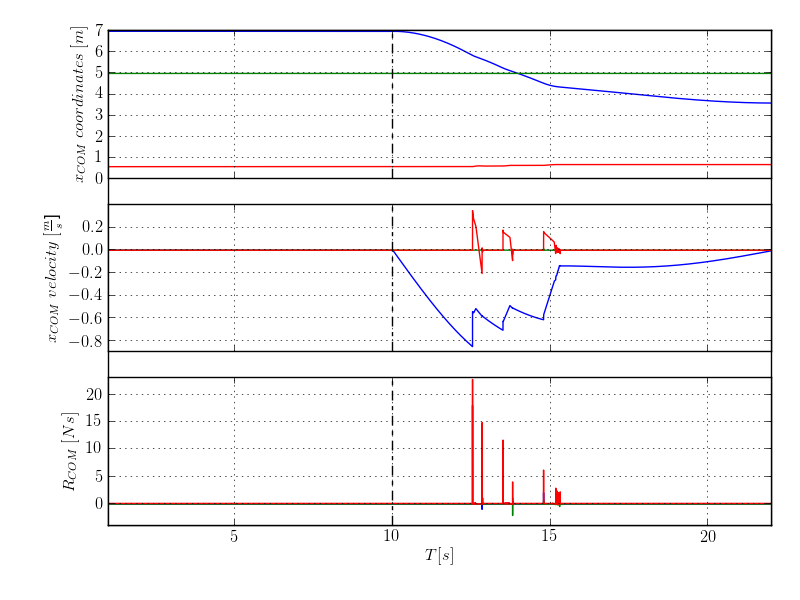
\includegraphics[width=0.8\textwidth]{xvpCOM7}
  \caption{$x_{COM}$ - mass center coordinates}
\end{figure}


\noindent \textbf{\textit{\Large{Comments}}}\\[1mm]
\noindent In the last setting the rover mounts a vertical step. Crossing of the obstacle occurs around $13^{th}$ second of the simulation then until the end of the simulation rover keeps moving on the upper plane. 
In the figure 31 one can see detailed motion of the rover when ascending and descending the step along all three coordinates of the mass center.
In the same figure, in the two last subplots one notices series of impacts corresponding to the impacts. Namely, in the second sub-plot three impacts can be seen along the z coordinate which correspond to impacts of each pair of
wheels. Impacts are also seen in the third sub-plot depicting reaction forces acting on the mass center. 
